% Created by tikzDevice version 0.8.1 on 2015-05-29 07:00:40
% !TEX encoding = UTF-8 Unicode
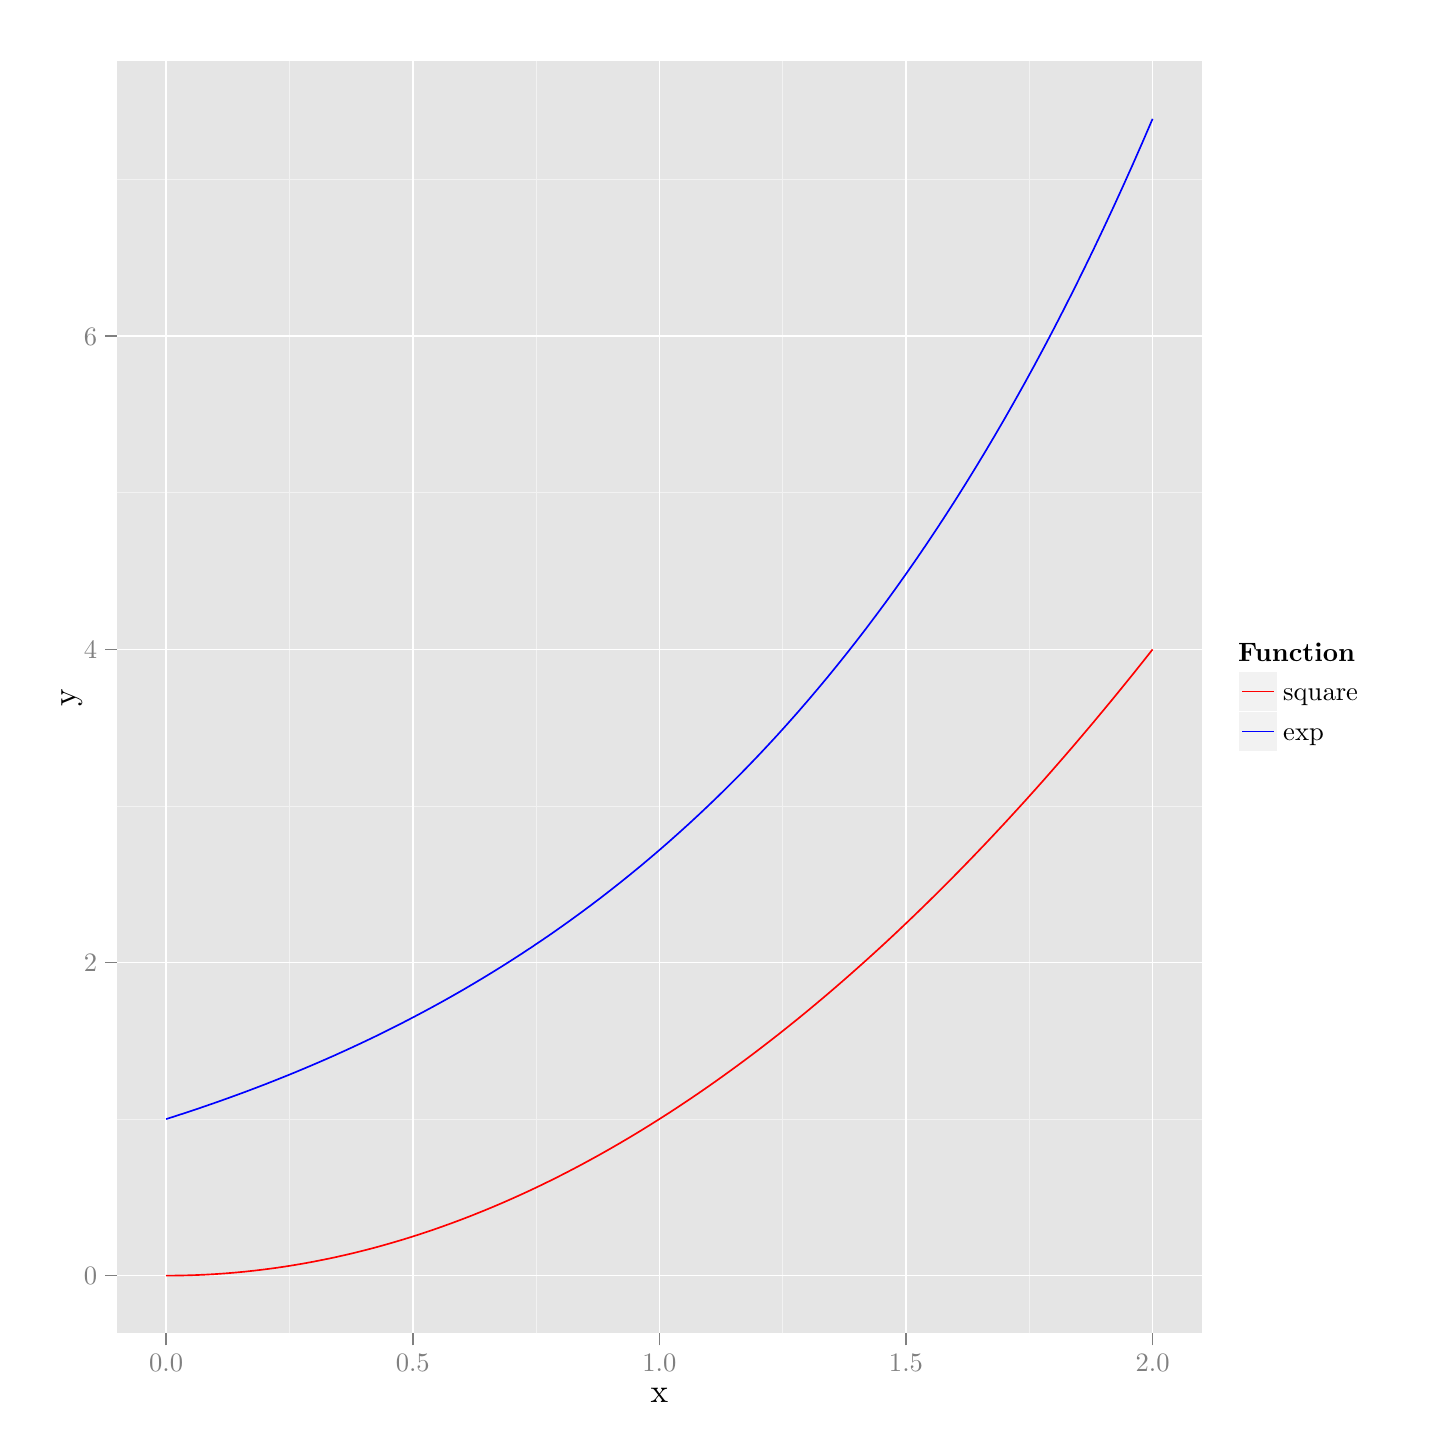
\begin{tikzpicture}[x=1pt,y=1pt]
\definecolor{fillColor}{RGB}{255,255,255}
\path[use as bounding box,fill=fillColor,fill opacity=0.00] (0,0) rectangle (505.89,505.89);
\begin{scope}
\path[clip] (  0.00,  0.00) rectangle (505.89,505.89);
\definecolor{drawColor}{RGB}{255,255,255}
\definecolor{fillColor}{RGB}{255,255,255}

\path[draw=drawColor,line width= 0.6pt,line join=round,line cap=round,fill=fillColor] (  0.00,  0.00) rectangle (505.89,505.89);
\end{scope}
\begin{scope}
\path[clip] ( 32.22, 34.03) rectangle (424.31,493.85);
\definecolor{fillColor}{gray}{0.90}

\path[fill=fillColor] ( 32.22, 34.03) rectangle (424.31,493.85);
\definecolor{drawColor}{gray}{0.95}

\path[draw=drawColor,line width= 0.3pt,line join=round] ( 32.22,111.51) --
	(424.31,111.51);

\path[draw=drawColor,line width= 0.3pt,line join=round] ( 32.22,224.65) --
	(424.31,224.65);

\path[draw=drawColor,line width= 0.3pt,line join=round] ( 32.22,337.79) --
	(424.31,337.79);

\path[draw=drawColor,line width= 0.3pt,line join=round] ( 32.22,450.94) --
	(424.31,450.94);

\path[draw=drawColor,line width= 0.3pt,line join=round] ( 94.60, 34.03) --
	( 94.60,493.85);

\path[draw=drawColor,line width= 0.3pt,line join=round] (183.71, 34.03) --
	(183.71,493.85);

\path[draw=drawColor,line width= 0.3pt,line join=round] (272.82, 34.03) --
	(272.82,493.85);

\path[draw=drawColor,line width= 0.3pt,line join=round] (361.93, 34.03) --
	(361.93,493.85);
\definecolor{drawColor}{RGB}{255,255,255}

\path[draw=drawColor,line width= 0.6pt,line join=round] ( 32.22, 54.94) --
	(424.31, 54.94);

\path[draw=drawColor,line width= 0.6pt,line join=round] ( 32.22,168.08) --
	(424.31,168.08);

\path[draw=drawColor,line width= 0.6pt,line join=round] ( 32.22,281.22) --
	(424.31,281.22);

\path[draw=drawColor,line width= 0.6pt,line join=round] ( 32.22,394.36) --
	(424.31,394.36);

\path[draw=drawColor,line width= 0.6pt,line join=round] ( 50.04, 34.03) --
	( 50.04,493.85);

\path[draw=drawColor,line width= 0.6pt,line join=round] (139.15, 34.03) --
	(139.15,493.85);

\path[draw=drawColor,line width= 0.6pt,line join=round] (228.26, 34.03) --
	(228.26,493.85);

\path[draw=drawColor,line width= 0.6pt,line join=round] (317.37, 34.03) --
	(317.37,493.85);

\path[draw=drawColor,line width= 0.6pt,line join=round] (406.48, 34.03) --
	(406.48,493.85);
\definecolor{drawColor}{RGB}{255,0,0}

\path[draw=drawColor,line width= 0.6pt,line join=round] ( 50.04, 54.94) --
	( 53.61, 54.96) --
	( 57.17, 55.03) --
	( 60.74, 55.14) --
	( 64.30, 55.30) --
	( 67.87, 55.50) --
	( 71.43, 55.75) --
	( 74.99, 56.04) --
	( 78.56, 56.38) --
	( 82.12, 56.77) --
	( 85.69, 57.20) --
	( 89.25, 57.67) --
	( 92.82, 58.19) --
	( 96.38, 58.76) --
	( 99.95, 59.37) --
	(103.51, 60.03) --
	(107.07, 60.73) --
	(110.64, 61.47) --
	(114.20, 62.27) --
	(117.77, 63.10) --
	(121.33, 63.99) --
	(124.90, 64.91) --
	(128.46, 65.89) --
	(132.02, 66.91) --
	(135.59, 67.97) --
	(139.15, 69.08) --
	(142.72, 70.23) --
	(146.28, 71.43) --
	(149.85, 72.68) --
	(153.41, 73.97) --
	(156.98, 75.30) --
	(160.54, 76.68) --
	(164.10, 78.11) --
	(167.67, 79.58) --
	(171.23, 81.09) --
	(174.80, 82.66) --
	(178.36, 84.26) --
	(181.93, 85.91) --
	(185.49, 87.61) --
	(189.06, 89.35) --
	(192.62, 91.14) --
	(196.18, 92.97) --
	(199.75, 94.85) --
	(203.31, 96.78) --
	(206.88, 98.74) --
	(210.44,100.76) --
	(214.01,102.82) --
	(217.57,104.92) --
	(221.14,107.07) --
	(224.70,109.27) --
	(228.26,111.51) --
	(231.83,113.79) --
	(235.39,116.12) --
	(238.96,118.50) --
	(242.52,120.92) --
	(246.09,123.39) --
	(249.65,125.90) --
	(253.21,128.46) --
	(256.78,131.06) --
	(260.34,133.71) --
	(263.91,136.40) --
	(267.47,139.14) --
	(271.04,141.92) --
	(274.60,144.75) --
	(278.17,147.62) --
	(281.73,150.54) --
	(285.29,153.51) --
	(288.86,156.51) --
	(292.42,159.57) --
	(295.99,162.67) --
	(299.55,165.82) --
	(303.12,169.01) --
	(306.68,172.24) --
	(310.25,175.52) --
	(313.81,178.85) --
	(317.37,182.22) --
	(320.94,185.64) --
	(324.50,189.10) --
	(328.07,192.61) --
	(331.63,196.16) --
	(335.20,199.76) --
	(338.76,203.40) --
	(342.32,207.09) --
	(345.89,210.82) --
	(349.45,214.60) --
	(353.02,218.43) --
	(356.58,222.30) --
	(360.15,226.21) --
	(363.71,230.17) --
	(367.28,234.18) --
	(370.84,238.23) --
	(374.40,242.32) --
	(377.97,246.46) --
	(381.53,250.65) --
	(385.10,254.88) --
	(388.66,259.16) --
	(392.23,263.48) --
	(395.79,267.85) --
	(399.36,272.26) --
	(402.92,276.72) --
	(406.48,281.22);
\definecolor{drawColor}{RGB}{0,0,255}

\path[draw=drawColor,line width= 0.6pt,line join=round] ( 50.04,111.51) --
	( 53.61,112.65) --
	( 57.17,113.82) --
	( 60.74,115.00) --
	( 64.30,116.22) --
	( 67.87,117.46) --
	( 71.43,118.72) --
	( 74.99,120.01) --
	( 78.56,121.32) --
	( 82.12,122.66) --
	( 85.69,124.03) --
	( 89.25,125.43) --
	( 92.82,126.85) --
	( 96.38,128.30) --
	( 99.95,129.79) --
	(103.51,131.30) --
	(107.07,132.84) --
	(110.64,134.41) --
	(114.20,136.02) --
	(117.77,137.66) --
	(121.33,139.33) --
	(124.90,141.03) --
	(128.46,142.77) --
	(132.02,144.55) --
	(135.59,146.36) --
	(139.15,148.21) --
	(142.72,150.09) --
	(146.28,152.01) --
	(149.85,153.97) --
	(153.41,155.97) --
	(156.98,158.01) --
	(160.54,160.10) --
	(164.10,162.22) --
	(167.67,164.39) --
	(171.23,166.60) --
	(174.80,168.86) --
	(178.36,171.16) --
	(181.93,173.51) --
	(185.49,175.90) --
	(189.06,178.34) --
	(192.62,180.84) --
	(196.18,183.38) --
	(199.75,185.98) --
	(203.31,188.62) --
	(206.88,191.32) --
	(210.44,194.08) --
	(214.01,196.89) --
	(217.57,199.76) --
	(221.14,202.68) --
	(224.70,205.67) --
	(228.26,208.71) --
	(231.83,211.82) --
	(235.39,214.99) --
	(238.96,218.22) --
	(242.52,221.52) --
	(246.09,224.89) --
	(249.65,228.32) --
	(253.21,231.82) --
	(256.78,235.39) --
	(260.34,239.04) --
	(263.91,242.76) --
	(267.47,246.55) --
	(271.04,250.42) --
	(274.60,254.37) --
	(278.17,258.40) --
	(281.73,262.51) --
	(285.29,266.71) --
	(288.86,270.98) --
	(292.42,275.35) --
	(295.99,279.80) --
	(299.55,284.34) --
	(303.12,288.98) --
	(306.68,293.71) --
	(310.25,298.53) --
	(313.81,303.45) --
	(317.37,308.47) --
	(320.94,313.59) --
	(324.50,318.82) --
	(328.07,324.15) --
	(331.63,329.59) --
	(335.20,335.14) --
	(338.76,340.80) --
	(342.32,346.57) --
	(345.89,352.46) --
	(349.45,358.47) --
	(353.02,364.60) --
	(356.58,370.86) --
	(360.15,377.24) --
	(363.71,383.75) --
	(367.28,390.40) --
	(370.84,397.17) --
	(374.40,404.09) --
	(377.97,411.14) --
	(381.53,418.34) --
	(385.10,425.68) --
	(388.66,433.17) --
	(392.23,440.81) --
	(395.79,448.60) --
	(399.36,456.55) --
	(402.92,464.67) --
	(406.48,472.94);
\end{scope}
\begin{scope}
\path[clip] (  0.00,  0.00) rectangle (505.89,505.89);
\definecolor{drawColor}{gray}{0.50}

\node[text=drawColor,anchor=base east,inner sep=0pt, outer sep=0pt, scale=  0.96] at ( 25.11, 51.63) {0};

\node[text=drawColor,anchor=base east,inner sep=0pt, outer sep=0pt, scale=  0.96] at ( 25.11,164.77) {2};

\node[text=drawColor,anchor=base east,inner sep=0pt, outer sep=0pt, scale=  0.96] at ( 25.11,277.91) {4};

\node[text=drawColor,anchor=base east,inner sep=0pt, outer sep=0pt, scale=  0.96] at ( 25.11,391.06) {6};
\end{scope}
\begin{scope}
\path[clip] (  0.00,  0.00) rectangle (505.89,505.89);
\definecolor{drawColor}{gray}{0.50}

\path[draw=drawColor,line width= 0.6pt,line join=round] ( 27.95, 54.94) --
	( 32.22, 54.94);

\path[draw=drawColor,line width= 0.6pt,line join=round] ( 27.95,168.08) --
	( 32.22,168.08);

\path[draw=drawColor,line width= 0.6pt,line join=round] ( 27.95,281.22) --
	( 32.22,281.22);

\path[draw=drawColor,line width= 0.6pt,line join=round] ( 27.95,394.36) --
	( 32.22,394.36);
\end{scope}
\begin{scope}
\path[clip] (  0.00,  0.00) rectangle (505.89,505.89);
\definecolor{drawColor}{gray}{0.50}

\path[draw=drawColor,line width= 0.6pt,line join=round] ( 50.04, 29.77) --
	( 50.04, 34.03);

\path[draw=drawColor,line width= 0.6pt,line join=round] (139.15, 29.77) --
	(139.15, 34.03);

\path[draw=drawColor,line width= 0.6pt,line join=round] (228.26, 29.77) --
	(228.26, 34.03);

\path[draw=drawColor,line width= 0.6pt,line join=round] (317.37, 29.77) --
	(317.37, 34.03);

\path[draw=drawColor,line width= 0.6pt,line join=round] (406.48, 29.77) --
	(406.48, 34.03);
\end{scope}
\begin{scope}
\path[clip] (  0.00,  0.00) rectangle (505.89,505.89);
\definecolor{drawColor}{gray}{0.50}

\node[text=drawColor,anchor=base,inner sep=0pt, outer sep=0pt, scale=  0.96] at ( 50.04, 20.31) {0.0};

\node[text=drawColor,anchor=base,inner sep=0pt, outer sep=0pt, scale=  0.96] at (139.15, 20.31) {0.5};

\node[text=drawColor,anchor=base,inner sep=0pt, outer sep=0pt, scale=  0.96] at (228.26, 20.31) {1.0};

\node[text=drawColor,anchor=base,inner sep=0pt, outer sep=0pt, scale=  0.96] at (317.37, 20.31) {1.5};

\node[text=drawColor,anchor=base,inner sep=0pt, outer sep=0pt, scale=  0.96] at (406.48, 20.31) {2.0};
\end{scope}
\begin{scope}
\path[clip] (  0.00,  0.00) rectangle (505.89,505.89);
\definecolor{drawColor}{RGB}{0,0,0}

\node[text=drawColor,anchor=base,inner sep=0pt, outer sep=0pt, scale=  1.20] at (228.26,  9.03) {x};
\end{scope}
\begin{scope}
\path[clip] (  0.00,  0.00) rectangle (505.89,505.89);
\definecolor{drawColor}{RGB}{0,0,0}

\node[text=drawColor,rotate= 90.00,anchor=base,inner sep=0pt, outer sep=0pt, scale=  1.20] at ( 17.30,263.94) {y};
\end{scope}
\begin{scope}
\path[clip] (  0.00,  0.00) rectangle (505.89,505.89);
\definecolor{fillColor}{RGB}{255,255,255}

\path[fill=fillColor] (433.17,240.10) rectangle (484.98,287.78);
\end{scope}
\begin{scope}
\path[clip] (  0.00,  0.00) rectangle (505.89,505.89);
\definecolor{drawColor}{RGB}{0,0,0}

\node[text=drawColor,anchor=base west,inner sep=0pt, outer sep=0pt, scale=  0.96] at (437.44,276.89) {\bfseries Function};
\end{scope}
\begin{scope}
\path[clip] (  0.00,  0.00) rectangle (505.89,505.89);
\definecolor{drawColor}{RGB}{255,255,255}
\definecolor{fillColor}{gray}{0.95}

\path[draw=drawColor,line width= 0.6pt,line join=round,line cap=round,fill=fillColor] (437.44,258.82) rectangle (451.90,273.27);
\end{scope}
\begin{scope}
\path[clip] (  0.00,  0.00) rectangle (505.89,505.89);
\definecolor{drawColor}{RGB}{255,0,0}

\path[draw=drawColor,line width= 0.6pt,line join=round] (438.89,266.05) -- (450.45,266.05);
\end{scope}
\begin{scope}
\path[clip] (  0.00,  0.00) rectangle (505.89,505.89);
\definecolor{drawColor}{RGB}{255,0,0}

\path[draw=drawColor,line width= 0.6pt,line join=round] (438.89,266.05) -- (450.45,266.05);
\end{scope}
\begin{scope}
\path[clip] (  0.00,  0.00) rectangle (505.89,505.89);
\definecolor{drawColor}{RGB}{255,255,255}
\definecolor{fillColor}{gray}{0.95}

\path[draw=drawColor,line width= 0.6pt,line join=round,line cap=round,fill=fillColor] (437.44,244.37) rectangle (451.90,258.82);
\end{scope}
\begin{scope}
\path[clip] (  0.00,  0.00) rectangle (505.89,505.89);
\definecolor{drawColor}{RGB}{0,0,255}

\path[draw=drawColor,line width= 0.6pt,line join=round] (438.89,251.59) -- (450.45,251.59);
\end{scope}
\begin{scope}
\path[clip] (  0.00,  0.00) rectangle (505.89,505.89);
\definecolor{drawColor}{RGB}{0,0,255}

\path[draw=drawColor,line width= 0.6pt,line join=round] (438.89,251.59) -- (450.45,251.59);
\end{scope}
\begin{scope}
\path[clip] (  0.00,  0.00) rectangle (505.89,505.89);
\definecolor{drawColor}{RGB}{0,0,0}

\node[text=drawColor,anchor=base west,inner sep=0pt, outer sep=0pt, scale=  0.96] at (453.70,262.74) {square};
\end{scope}
\begin{scope}
\path[clip] (  0.00,  0.00) rectangle (505.89,505.89);
\definecolor{drawColor}{RGB}{0,0,0}

\node[text=drawColor,anchor=base west,inner sep=0pt, outer sep=0pt, scale=  0.96] at (453.70,248.29) {exp};
\end{scope}
\end{tikzpicture}
